\documentclass[11pt,a4paper]{article}
\usepackage[T1]{fontenc}
\usepackage[utf8]{inputenc}
\usepackage{lmodern}
\usepackage{amsmath,amssymb}
\usepackage{booktabs}
\usepackage{graphicx}
\usepackage[margin=2.2cm]{geometry}
\usepackage[colorlinks=true,linkcolor=blue,citecolor=blue,urlcolor=blue]{hyperref}

\newcommand{\code}[1]{\texttt{#1}}

\title{Ten-day dry baroclinic wave with CGSEM and DGSEM\\[0.3em]
\large Short version: setups, time step, final timings and accuracy}
\author{CGDycore.jl}
\date{\today}

\begin{document}
\sloppy
\maketitle

\noindent This is a summary of \code{BaroWave10Days.tex}, which gives the
details, the kernel work on DGSEM and the reproduction scripts. All timings
here are from ten-day runs with the final code on one NVIDIA A100-SXM4-80GB
on Levante, without output.

\section{Test case and models}

The test is the dry baroclinic wave (\code{--Problem=BaroWaveDrySphere}):
flat ground, model top at 30~km, Earth radius and rotation, no damping
layer and no forcing, ten simulated days.

\begin{itemize}
\item \textbf{CGSEM} (CGDycore.jl, continuous Galerkin), job file
  \code{Jobs/NHSphere/CG/BaroWaveDrySphere\_32Elem}: cubed sphere,
  order~3, 64 stretched layers with vertically linear elements,
  vector-invariant momentum equation, shallow-atmosphere equations,
  vertical upwinding, fourth-order hyperviscosity
  $5\cdot10^{14}\,\mathrm{m^4\,s^{-1}}$. A second run uses the
  deep-atmosphere equations. CG-A and CG-B are order-4 variants with the
  deep equations: CG-A on the DGSEM element grid, CG-B with about the
  number of unknowns of DGSEM.
\item \textbf{DGSEM} (CGDycore.jl, discontinuous Galerkin), job files
  \code{Jobs/NHSphere/DG/BaroWaveDrySphereDGQuad*}: cubed sphere,
  order~4 horizontally and vertically, deep-atmosphere equations with the
  full Coriolis term, Cartesian velocity components, no explicit
  diffusion. Three flux pairs: \textbf{VI} (vector-invariant),
  \textbf{Cons} (conservative, Kennedy--Gruber with LMARS) and
  \textbf{Diff} (conservative, pressure as a difference to a reference
  state). VI is also run on prisms (icosahedral grid refined four times,
  5120 triangles, order~4, 13 vertical elements of order~4).
\item \textbf{ClimaAtmos.jl} v0.42.18 on the CGSEM grid: CG spectral
  elements on ClimaCore, staggered finite differences vertically, shallow
  atmosphere, default hyperdiffusion, minimal dry configuration without
  diagnostics and output.
\item \textbf{TrixiAtmo.jl} (commit 5874d5f, Trixi.jl v0.18.1-DEV) on the
  DGSEM grid: potential-temperature form, entropy-conservative volume flux,
  LMARS surface flux, on the GPU without callbacks.
\end{itemize}

\noindent\textbf{Reference:} DGSEM VI in Float64 with twice the resolution
in both directions ($n_\text{Panel}=40$, 26 vertical elements,
$\Delta t=42.5$~s). It favours DGSEM, since it is itself a DGSEM run.

\section{Resolution}

The spacing is measured along a panel edge; the smallest node distance is
the first GLL gap of the element at the panel centre on the equator.

\begin{center}
\small\setlength{\tabcolsep}{4pt}
\begin{tabular}{lrrrrrr}
\toprule
 & $n_\text{Panel}$ & $N$ & columns & vertical & mean / min & unknowns \\
 & & & & nodes & $\Delta x$ & per variable \\
\midrule
CGSEM standard, ClimaAtmos & 32 & 3 & 55\,298 & 64 & 104 / 86 km & 3.54\,M \\
CG-A           & 20 & 4 & 38\,402 & 52 & 125 / 86 km & 2.00\,M \\
CG-B           & 25 & 4 & 60\,002 & 65 & 100 / 69 km & 3.90\,M \\
DGSEM, TrixiAtmo & 20 & 4 & 60\,000 & $13\times5=65$ & 100 / 86 km & 3.90\,M \\
DGSEM reference & 40 & 4 & 240\,000 & $26\times5=130$ & 50 / 43 km & 31.2\,M \\
\bottomrule
\end{tabular}
\end{center}

\section{Time stepping}

All CGDycore runs use the three-stage Rosenbrock W-method \code{SSP-Knoth}.
The W-matrix holds only the vertical acoustic and gravity terms, so the
scheme is horizontally explicit and vertically linearly implicit (HEVI).
CGSEM solves the column systems directly; DGSEM condenses them onto the
element interfaces of each column (HDG). ClimaAtmos uses its IMEX method
ARS343 (four explicit and three implicit stages, one Newton iteration per
implicit stage, one Jacobian per step). TrixiAtmo uses the Rosenbrock-W
method \code{SSPRW32} with a two-sided vertical Schur-complement solver.

The time step is the largest stable one, limited by the horizontal Courant
number $C=c\,\Delta t/\Delta x_\text{min}$ with $c=340$~m/s:

\begin{center}
\small
\begin{tabular}{lrrl}
\toprule
 & $\Delta t$ [s] & $C$ & larger step \\
\midrule
CGSEM standard, CG-A, ClimaAtmos & 150 & 0.59 & 225--300 s: NaN within one day \\
CG-B           & 120 & 0.59 & \\
DGSEM, TrixiAtmo & 85 & 0.33 & \\
DGSEM prisms   & 75  & & \\
\bottomrule
\end{tabular}
\end{center}

\noindent CGSEM is stable at $C=0.59$, DGSEM at $C=0.33$. For the same
smallest node distance CGSEM takes a 1.8 times larger step. The
baroclinic-wave job file of CGSEM sets $\Delta t=230$~s, which is
unstable.

\section{Final timings and accuracy}

Wall time of the ten days without the first step (compilation),
SYPD $=(10/365)/(t_\text{wall}/86400)$. The error is the rms difference of
the day-10 surface pressure against the reference on a $0.5^\circ$ grid up
to $85^\circ$N, weighted with $\cos\varphi$; the last column is the
rms difference between Float32 and Float64 of the same run.

\begin{center}
\footnotesize\setlength{\tabcolsep}{4pt}
\begin{tabular}{llrrrrrr}
\toprule
run & precision & steps & wall [s] & ms/step & SYPD & error [hPa] & F32$-$F64 [hPa] \\
\midrule
CGSEM standard (shallow) & Float32 & 5\,760 & 114.4 & 19.9 & 20.7 & 1.94 & 0.031 \\
CGSEM standard (shallow) & Float64 & 5\,760 & 212.7 & 36.9 & 11.1 & 1.94 & \\
CGSEM standard, deep     & Float64 & 5\,760 & 223.2 & 38.8 & 10.6 & 0.64 & \\
CG-A                     & Float32 & 5\,760 & 67.7  & 11.8 & 35.0 & 0.76 & 0.046 \\
CG-A                     & Float64 & 5\,760 & 120.7 & 21.0 & 19.6 & 0.76 & \\
CG-B                     & Float32 & 7\,200 & 161.7 & 22.5 & 14.6 & 0.58 & 0.043 \\
CG-B                     & Float64 & 7\,200 & 280.6 & 39.0 & 8.4  & 0.59 & \\
\midrule
DGSEM VI                 & Float32 & 10\,165 & 100.4 & 9.9  & \textbf{23.6} & 0.41 & 0.059 \\
DGSEM VI                 & Float64 & 10\,165 & 161.1 & 15.8 & 14.7 & 0.41 & \\
DGSEM Cons               & Float32 & 10\,165 & 94.3  & 9.3  & 25.1 & 2.80 & 2.75 \\
DGSEM Cons               & Float64 & 10\,165 & 145.8 & 14.3 & 16.2 & 0.40 & \\
DGSEM Diff               & Float32 & 10\,165 & 93.9  & 9.2  & 25.2 & 0.41 & 0.070 \\
DGSEM Diff               & Float64 & 10\,165 & 145.9 & 14.4 & 16.2 & 0.40 & \\
DGSEM VI, prisms         & Float32 & 11\,520 & 110.5 & 9.6  & 21.4 & 0.70 & 0.106 \\
DGSEM VI, prisms         & Float64 & 11\,520 & 186.8 & 16.2 & 12.7 & 0.70 & \\
\midrule
ClimaAtmos               & Float32 & 5\,760 & 596.3  & 103.5 & 3.97 & 1.09 & 0.089 \\
ClimaAtmos               & Float64 & 5\,760 & 1347.6 & 234.0 & 1.76 & 1.09 & \\
TrixiAtmo                & Float32 & 10\,165 & 104.8 & 10.3 & 22.6 & 1.09 & 1.05 \\
TrixiAtmo                & Float64 & 10\,165 & 176.8 & 17.4 & 13.4 & 0.45 & \\
\bottomrule
\end{tabular}
\end{center}

\noindent ClimaAtmos stores no surface pressure; it is extrapolated from
the lowest level and shifted by $-13.25$~hPa, because its baroclinic wave
uses a sea-level pressure of 1013.25~hPa. The ClimaAtmos and TrixiAtmo
runs are those of the long document; the CGSEM and DGSEM runs were all
repeated with the final code (the CGSEM runs are 2--8\,\% faster than
before, probably from the fused stage copy of the Rosenbrock integrator).

\section{Findings}

\begin{itemize}
\item \textbf{Cost at the same number of unknowns.} DGSEM VI and CG-B both
  have 3.9\,M unknowns per variable. DGSEM takes 1.4 times more steps, but
  each costs 2.3 times less (9.9 against 22.5~ms in Float32). DGSEM VI
  therefore reaches 23.6~SYPD at 0.41~hPa, against 14.6~SYPD at
  0.58~hPa for CG-B.
\item \textbf{Standard setups.} The CGSEM job (order~3,
  $n_\text{Panel}=32$) reaches 20.7~SYPD in Float32 and DGSEM VI 23.6.
  CG-A is the fastest run (35.0~SYPD), but it has only 2.0\,M unknowns and
  an error of 0.76~hPa.
\item \textbf{Accuracy.} All DGSEM flux pairs on quadrilaterals are within
  0.40--0.41~hPa of the reference (except Cons in Float32). CGSEM is
  within 0.58--0.76~hPa with the deep-atmosphere equations. The shallow
  standard CGSEM job adds an almost uniform 1--2~hPa offset against the
  deep reference (1.94~hPa). The prisms are less accurate (0.70~hPa).
\item \textbf{Float32.} Float32 is 1.5--1.9 times faster than Float64. It
  keeps the Float64 accuracy for CGSEM, ClimaAtmos and DGSEM VI and Diff
  (Float32 error at most a sixth of the error against the reference). The
  conservative fluxes with the full pressure $p\approx10^5$~Pa fail in
  Float32: DGSEM Cons develops a spurious wave train (2.8~hPa), and
  TrixiAtmo, which also carries the full pressure, loses accuracy
  (1.09 against 0.45~hPa). The vector-invariant form with the Exner
  pressure and the difference form avoid this.
\item \textbf{External codes.} DGSEM VI is 4\,\% (Float32) and 10\,\%
  (Float64) faster than TrixiAtmo on the same grid and step, and in
  Float32 as accurate as TrixiAtmo in Float64 while 1.8 times faster.
  ClimaAtmos is far slower (next section).
\item \textbf{Reproducibility.} The DGSEM kernels use no atomics, so
  repeated runs give bitwise identical results.
\end{itemize}

\section{Why ClimaAtmos is slower}

On the same grid and with the same time step as the standard CGSEM run,
ClimaAtmos is 5.2 (Float32) and 6.3 (Float64) times slower per step. A kernel profile
of five Float32 steps (\code{CUDA.@profile}, 107~ms per step) shows:

\begin{itemize}
\item \textbf{Not launch-bound.} The GPU is busy 96\,\% of the time; the
  host mostly waits in \code{cuStreamSynchronize}.
\item \textbf{Many small kernels.} About 512 kernel launches per step
  (107 different kernels), against about 47 in DGSEM. ClimaCore turns each
  fused broadcast or column operator into its own kernel, and every stage
  recomputes the full cache of diagnostic fields (thermodynamic state,
  kinetic energy, contravariant velocities, pressure). The prognostic
  total energy $\rho e_\text{tot}$ makes recovering temperature and
  pressure more expensive.
\item \textbf{Column kernels dominate.} The largest kernel, a vertical
  finite-difference column operator, takes 1.5~ms per call, 12 calls per
  step, 17\,\% of the time.
\item \textbf{More function evaluations.} ARS343 needs four explicit and
  three implicit tendency evaluations and three Newton solves per step,
  \code{SSP-Knoth} three tendency evaluations and one Jacobian.
\item \textbf{The Jacobian is not the cost.} Building it once per step
  instead of once per solve changes the step time by 2\,\%; the
  tridiagonal solve takes less than 1\,\%.
\item \textbf{Generality.} The dry dycore runs through the code paths of
  the full model (moisture, EDMF and tracer machinery switched off but
  still structuring state and cache). A substantial speed-up would need
  fewer, fused kernels in ClimaCore and ClimaAtmos, not a different
  configuration: removing diagnostics and output changed the Float64 step
  only from 0.239 to 0.234~s.
\end{itemize}

\noindent Float32 works in ClimaAtmos (0.09~hPa rms against Float64) and
halves the cost.

\begin{figure}[p]
\centering
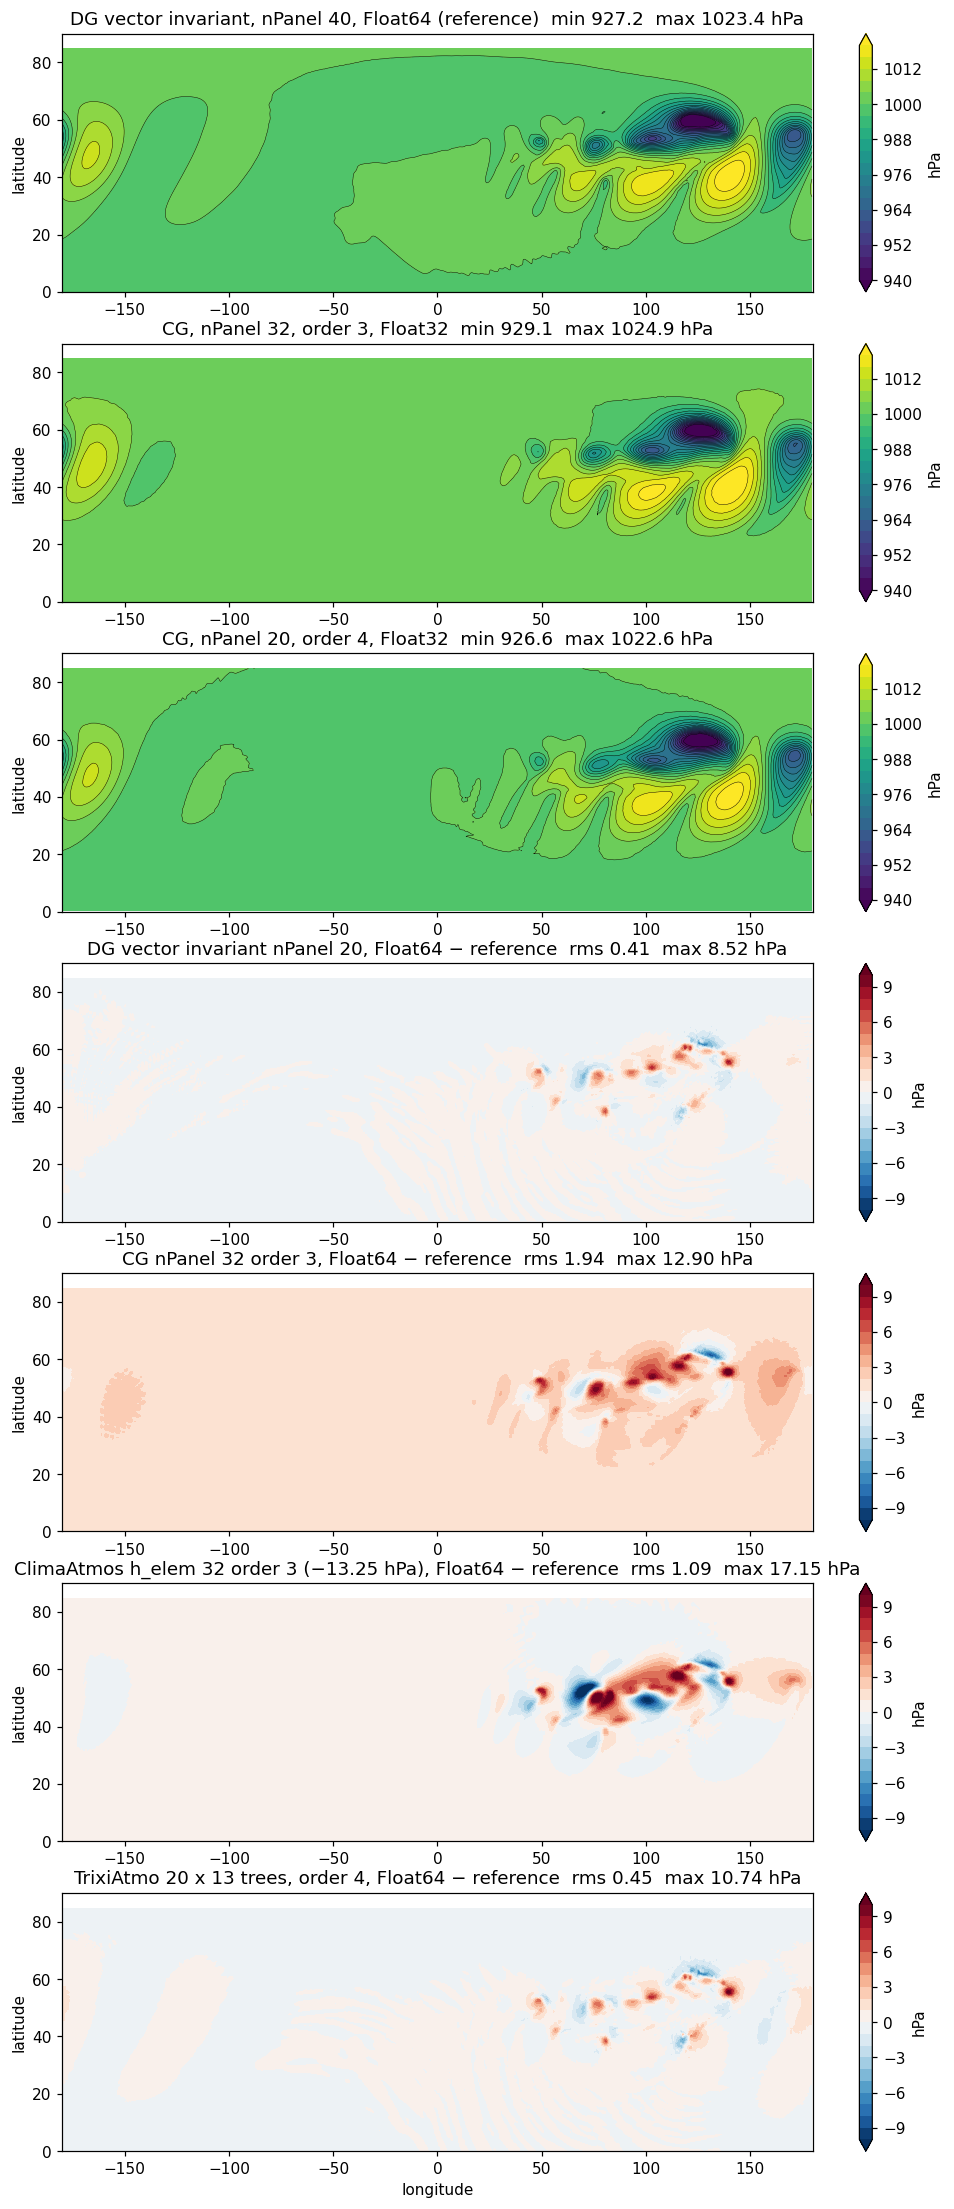
\includegraphics[height=0.8\textheight,keepaspectratio]{BaroWave10Days_ps.png}
\caption{Day-10 surface pressure: DGSEM VI reference ($n_\text{Panel}=40$),
CGSEM standard (order 3, $n_\text{Panel}=32$, shallow) and CG-A (order 4,
$n_\text{Panel}=20$) in Float32, and the Float64 differences of DGSEM VI,
CGSEM standard, ClimaAtmos (shifted by $-13.25$~hPa) and TrixiAtmo
against the reference.}
\label{fig:all}
\end{figure}

\end{document}
